\section{Results}
%Maintain past tenses for results obtaiend!!

\subsection{Deterministic LP}
The simplified approach represented nothing but a upper-bound of the more realistic one. Indeed, as HRT was computed from the results of the simplified-LP, the constraint for HRT$_{min}$ was always active (the higher the inflow rate, the higher the profit if no realistic worsening effects on the productivity resulting from a low HRT are considered).
It was interesting to note that, running the realistic-LP with HRT=$+\infty$, the solution suggested the same diet of the simplified-LP, whereas setting HRT=HRT$_{min}$ the suggested diet was different.
It can be concluded, as expected, that the diet with the highest conversion yield (i.e. BMP$_\infty$) is different from the one with the highest productivity (i.e. BMP at low HRT values), and that, under realistic approach, the profit was maximized adopting the one with the highest productivity.
As a result, the best profit was always obtained at the lowest feasible HRT (19 days), and that the latter may be higher only in case the constraint on BMP$_{res,max}$ is active and more restrictive (or similarly, some other possible constraints to avoid excessive residual organic matter in the effluent or the risk for reactor acidification). If no direct/indirect bounds on HRT is enforced, the best profit was achieved for HRT=4, that would for sure lead to reactor acidification, bacteria inhibition and consequent drop of the productivity (verification with ADM1).
This is due to the fact that, with the collected data and related BMP(HRT) curves, the objective function value was more sensitive to the quantity of purchased material than to the conversion yields, in the HRT range of practical interest. 
It is also important to highlight that the other operational expenditures that were neglected are inversely proportional to HRT (es. pumping cost, heating self-consumption, costs of digestate valorization or disposal).
Eventually, from expert knowledge we can state that the most interesting region for real plant operation is between 30-40 days.

Results from multiple realistic-LP runs at different HRT suggested a relevant and superlinear decrease in the profit with HRT, and an interesting shift in the diet composition, as shown in  Fig.\ref{fig:screeningHRTD}. 
In the HRT range of interest, 'maize silage' was the best cost-effective item to select, as also suggested by Fig.\ref{fig:netprofitbmp}. The extent of selection of 'maize silage' was defined by the feasible region, limited by the infleunt diet process and regulating authority constraints. In this case, 'maize silage' was always selected at the highest extension up to the 20\% regulating authority limit. At low HRT values, the extent of carbon-rich items in the diet was higher (+34.6\%) with respect to high HRT values. As they are characterized by faster degradation kinetic and higher BMP$_\infty$ with respect to slurries, this increased even further the difference between J values for low/high HRTs. Barley and triticale silages are thus selected to reach the upper limit on the exploitation of agri-products (P). 
It is important to highlight that slurries and dungs (S category) are forced to constitute a big percentage of the diet to fulfill both VS and regularing authority constraints ($\geq$ 70\%). Slurries are preferred over dungs because of their lower VS content: indeed, dungs present a conversion yield similar to slurries but with higher VS content that would limit the selection of silages, that are charcterized by higher unitary profit as shown in Fig.\ref{fig:netprofitbmp}.
It was interesting to note the shift from pig to cow slurry with increasing HRT: 'cow slurry' is more expensive, but it has also a higher BMP$_\infty$. 
Where possible, the problem tent to push toward the purchase of silages, and fulfill the other constraints with the more productive 'cow slurry'. Nevertheless, at high HRT, silages purchase was limited by the VS constraint on the diet: indeed, cow has higher VS content than pig slurry. In addition, the fixed amount of constrained 'cow dung' produced at the plant characterized by relatively high VS has a higher impact on this constraint at high HRT.
At low HRT the purchased quantities must be higher, so that it was chosen to move to the cheaper and lower-productive pig slurry and, thanks to the higher room for VS, increase the content of silages in the diet. 
Altought silages are more cost-effective than slurries, the J tent to be sensitive to slurries because their extent in the diet is forced to be always much higher than the other items for the VS and regulating authority constraints. The exploitation of other promising substrates such as 'wheat byproducts' and 'chicken dung' is probably hindered by their high TKN value.
Indeed, we remark that the active technical constraints are the VS (for all HRT values) and the TKN (for intermediate HRT values) ones.

Interestingly, intermediate HRTs result in a higher degree of diversification between the two slurries.

All the considerations based on the analysis of Fig.\ref{fig:netprofitbmp} are consistent also because of the small relevance of transportation costs in the distance range that was considered (0-50 km): indeed, they made up between 17-18\% of the total costs for all the HRT values. If the best items as identified by Fig.\ref{fig:netprofitbmp} were present only at very far away locations or if they were characterized by very high specific fixed transportation tariff, the considerations must be re-discussed. 

\begin{figure*}[htb]
 \begin{center}
  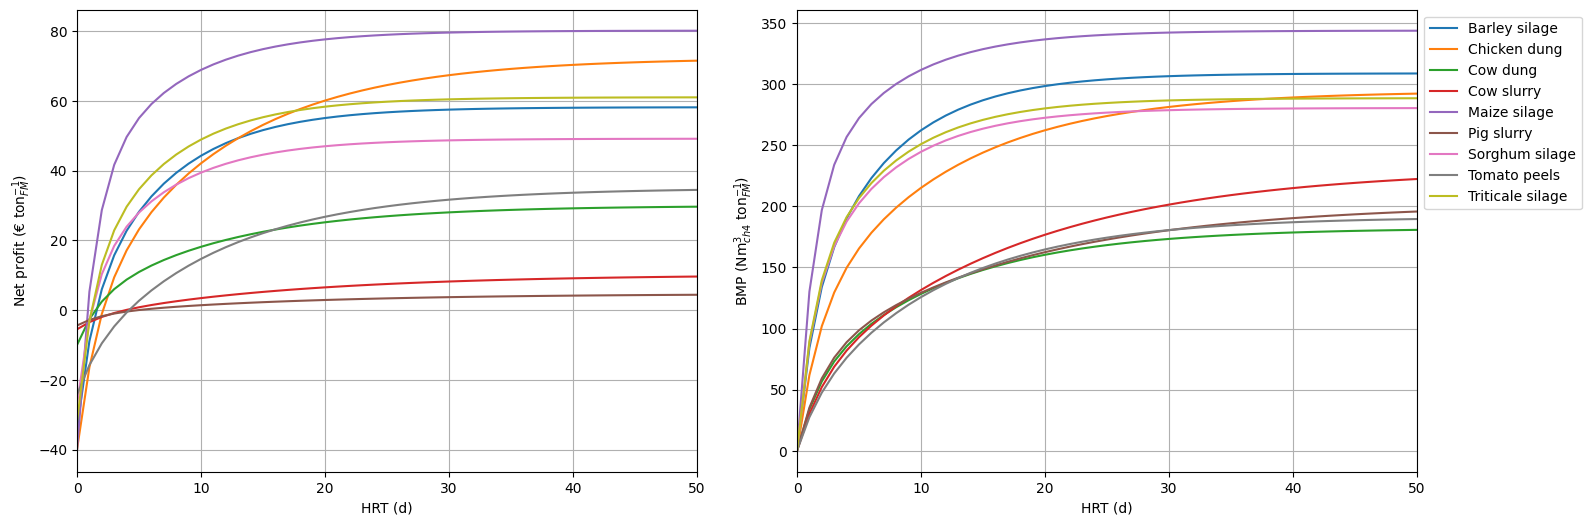
\includegraphics[width=2\columnwidth]{./img/NetProfitBMP_2024-05-02.png}
 \end{center}
 \caption{Comparison between the specific unitary profit (left) and BMP (right) of the different items. Here, the profit does not consider the transportation cost. 'Wheat by-products' is not shown, because out from the scale of interest. Unitary profit was computed as $p_{ch4} \times VS \times BMP(HRT) - C_p$}
 \label{fig:netprofitbmp}
\end{figure*}

\begin{figure*}[htb]
 \begin{center}
  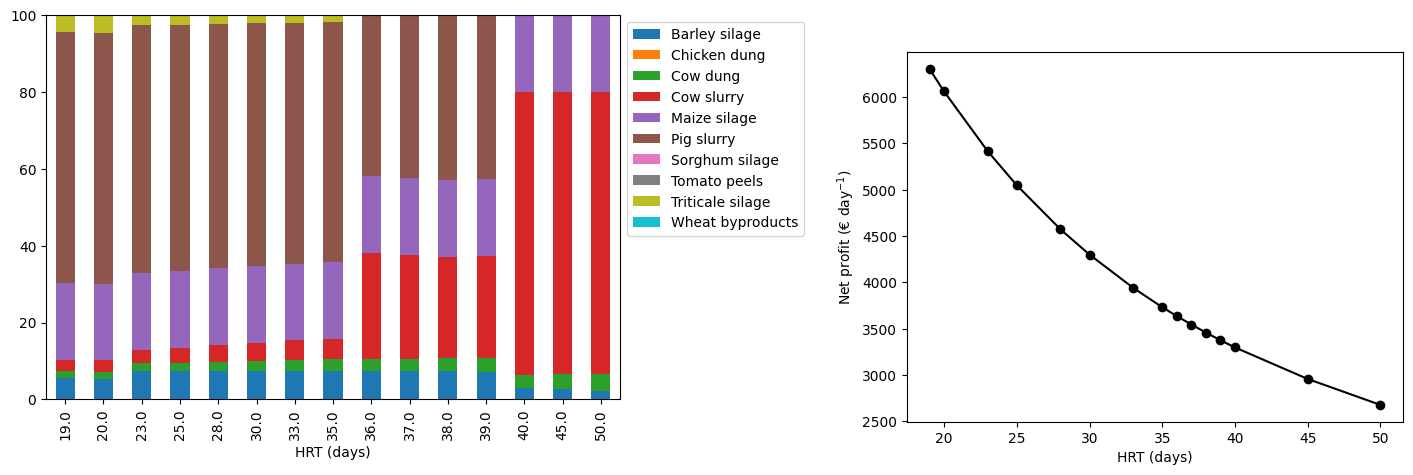
\includegraphics[width=2\columnwidth]{./img/Screening_HRT_D-LP_2024-05-02.png}
 \end{center}
 \caption{Comparison between LP solutions (left) and objective function values (right) obtained for different value of HRT}
 \label{fig:screeningHRTD}
\end{figure*}
%------------------------------------------------------------------------------------

\subsection{Robustified (R-) LP}

The introduction of availability uncertainty is not of particular interest, as the worst-case scenario for the problem under study is very likely to coincide to a realization for which all the item availabilities are equal to their lower-bound i.e. to a deterministic formulation with new bounds to matrix \emph{A}. As few of the availability constraints were active, enforcing uncertainty did not affect significantly the value of the profit ($\leq$ 1\%): this was due to the low impact of transportation costs for the less abundant and interesting items (i.e. silages), coupled with a small difference between transportation costs of the nearest and the second-nearest sellers. The impact could be more relevant for if data are generated with higher variance. The only difference in the diet composition was observed at low HRT, with a reduced purchase of 'triticale silage', substituted by 'barley silage' (triticale is slightly more cost-effective, but with a higher VS content).

The introduction of price uncertainty did impact the value of the profit of 14.4\% and 13.8\% for HRT equal to 20 and 50 respectively. Interestingly, the diet remained almost the same as for the deterministic solution, proving resiliance to price uncertainty of the optimal diet.

Similar considerations hold if only BMP$_\infty$ (and availability) uncertainty is introduced, although a higher impact was observed, as the profit dropped by 30.1\% and 26.9\% for HRT equal to 20 and 50 respectively.

When the two uncertainty sources were simultaneously introduced, the profit dropped by 44.5\% and 40.6\% for HRT equal to 20 and 50 respectively. This may suggest that operating a reactor with high HRT is only slightly more robust. Nevertheless, the absolute profit loss introduced by robustification is much higher for a rector with low HRT (148\%). 
It is important to note that the worst-case realization at HRT=20 still returned a slightly higher profit then the deterministic profit at HRT=50.

At HRT=50, some 'maize silage' was substituted with 'barley silage': this is most likely due to the higher maximum/mean ratio of the price of maize with respect to barley. It can be stated that barley is the safest alternative to maize.

The results of the screening for different HRT values screening are shown in Fig.\ref{fig:screeningHRTR}.
The standard deviation computed on the same HRT values for both the LP and R-LP J values suggested a lower variability (-28.6\%) with HRT for the robustified solutions. This also increases the "degree of robustness" of the solution obtained with the R-LP formulation. 

The differences in the diet compositions follow similar considerations as for the LP solutions was confirmed (es. barley as second-best and safer alternative to maize at high HRTs).
Nevertheless:
\begin{itemize}
    \item The shift from pig to cow slurry is moved to lower HRTs. Indeed, 'cow slurry' is a safer option than 'pig slurry' because of its lower max/mean ratio of the purchase price and higher min/mean ratio of the BMP$_\infty$;
    \item Less 'triticale silage' is available for purchase at low HRTs.
\end{itemize}

The values of the "nominal" size parameters for the uncertainty sets are reported in Table. 

\begin{figure*}[htb]
 \begin{center}
  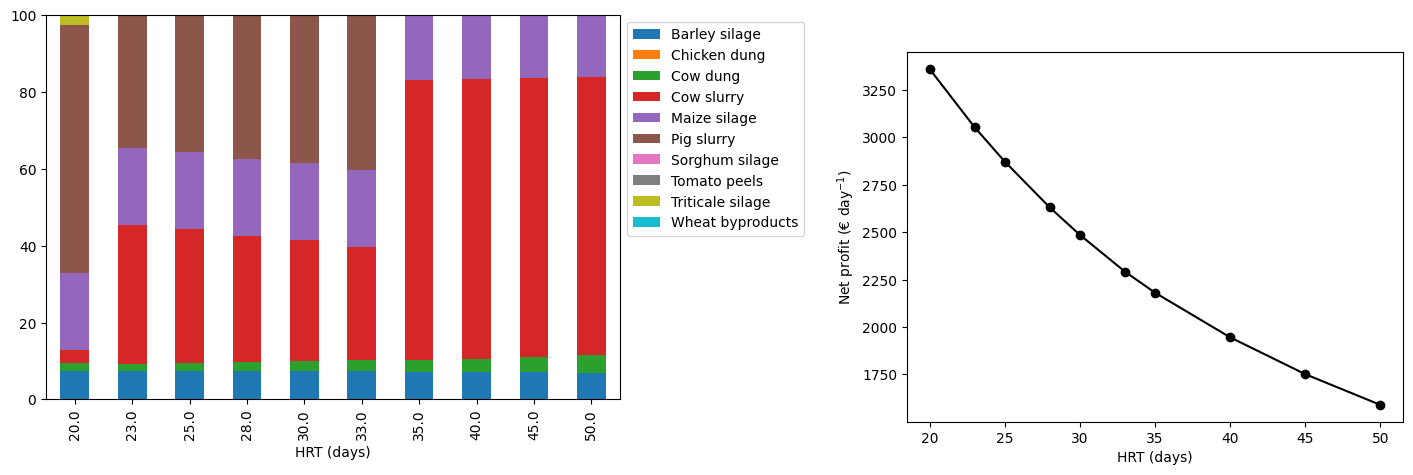
\includegraphics[width=2\columnwidth]{./img/Screening_HRT_R-LP_2024-05-02.png}
 \end{center}
 \caption{Comparison between R-LP solutions (left) and objective function values (right) obtained for different value of HRT}
 \label{fig:screeningHRTR}
\end{figure*}

After the model was solved with the "nominal/trained" value of Gamma\_price, some later testing was performed. Additional realization of price data were generated for the consequent remaining 20 years of future plant operation. For each realization, the value of J was computed taking the same values of decision variables obtained so far, for both a high and low HRT value (50 and 20 days respectively). The "nominal" J value was compared with the distribution of J obtained under testing price realizations and results are shown in Fig.\ref{fig:testing20}-\ref{fig:testing50}. It is important to stress out that this comparison was possible only under the same realization of availability and BMP$_\infty$: in this case, the deterministic values were considered.
The profit of the deterministic LP was found in line with the ones computed under testing realizations; nevertheless, it was slightly too optimistic, being higher than the average profit obtained in testing (few percentage points).
In contrary, the profit suggested by the R-LP looks overly conservative, being 11.9\% and 11.1\% lower than the profit value located at the "minimum" whisker of the box-plot, for HRT=20 and 50 respectively. 
From the width of the box-plots, it was also interesting to note the greater dispersion of the profit values at HRT=20 with respect to HRT=50, remarking the higher "safety degree" of reactors operated at high HRTs. 

\begin{figure}[htb]
 \begin{center}
  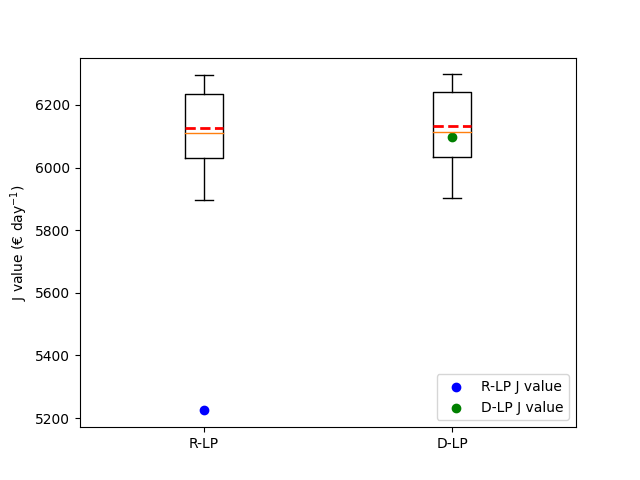
\includegraphics[width=1\columnwidth]{./img/Testing_20_2024-05-02.png}
 \end{center}
 \caption{Comparison between nominal and test objective function value for HRT=20}
 \label{fig:testing20}
\end{figure}

\begin{figure}[htb]
 \begin{center}
  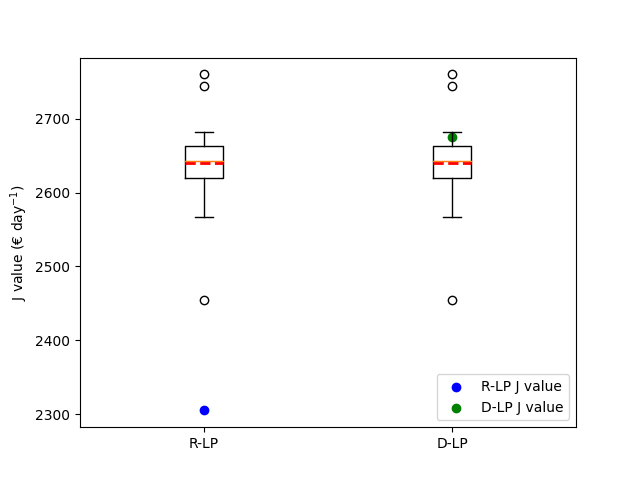
\includegraphics[width=1\columnwidth]{./img/Testing_50_2024-05-02.png}
 \end{center}
 \caption{Comparison between nominal and test objective function value for HRT=50}
 \label{fig:testing50}
\end{figure}
%------------------------------------------------------------------------------------

%\subsection{Unique $\mathbf{\Zeta}$ vs multiple $\Zeta$'s}
%------------------------------------------------------------------------------------

\subsection{Map of optimal solutions for different $\Gamma$}

Some analysis was carried out to assess the impact of the choice of the size parameters for the uncertainty sets. The aim was to provide decision-makers a map of the possible worst-case profits and diet compositions under different "risk degree" (Prob parameter). Table\ref{tab:gammas} reports the values investigated and the consequent values of the size parameters. The number of items that can simultaneously attain extreme values is highly impacted by the value of Prob, in particular for the BMP$_\infty$, coherently with the higher dispersion that Theorem 3.5 covers with respect to the lower variance of the availability and price distributions. 

Results are reported in Fig.\ref{fig:screenVaR20}-\ref{fig:screenVaR50}.

As far as the comparison between low and high HRT is concerned, the same observations on the higher variability of the profit with low HRT held.
Additionally, interesting differences in the diet composition were observed:
\begin{itemize}
    \item At high Prob, the value of the size parameters was bigger than the number of different items present in the diet. In the worst-case realization, both slurries could be at their worst performance (high price and low BMP$_\infty$), so that the one leading to the best worst-case was selected to cover all the diet percentage imposed by VS and regulating authority constraints. The choice of pig or cow at the different HRT followed the above-mentioned observations (es. at low HRT I have to buy more, so I choose the cheapest (pig) to fulfill constraints). When the size parameter was bigger than its nominal (Prob=95\%) value, nor J or the diet changed: this was still due to the fact that the size parameter became larger the the number of items present in the diet with in a relevant percentage i.e. able to affect J the most (3 or 4).
    \item At low Prob (Prob $\leq$ 20\% i.e. Gamma\_price $\leq$ 3 and Gamma\_BMP $\leq$ 2), a lower number of items ($\leq$ number of items relevant in the diet composition) could attain its worst-case, so that the tendency of the solver to diversify the diet was clearly observable.
    \item Interestingly, the J value at extremely low Prob is lower with respect to the deterministic profit for the same HRT. This could be partially due to a small deviation of \emph{$\mu_P$} from the deterministic purchase prices, but was primarily due to the relevant value of the price set size parameter (Gamma\_price $\geq$ 1.8). Indeed, this value was high enough to affect at their worst-case the most relevant items in the diet and thus impacting a low the profit.
    In addition, from Fig.\ref{fig:dataprice} we observe the (realistic) low range of variability of 'cow slurry' and 'pig slurry'. Due to this reason, after the most of the profit loss due to price extinguished at low Prob, the impact of only price uncertainty at higher values of Prob did not increases substantially (only 4.3\% profit drop from 1\% to 95\% Prob values, if only price (and availability) uncertainties were in place).
    \textcolor{red}{Consideration of intermediate values leading to more triticale than maize? Intermediate Prob similar to intermediate HRTs?}
\end{itemize}

% Table generated by Excel2LaTeX from sheet 'For Report'
\begin{table}[htbp]
  \centering
  \caption{Uncertainty set size parameters correspondent to different threshold of probability Prob to meet the change constraint}
    \begin{tabular}{ScScScSc}
    \toprule
    Prob & Gamma\_availability & Gamma\_price & Gamma\_BMP \\
    \midrule
    1\%   & 4.7   & 1.8   & 0.4 \\
    5\%   & 4.7   & 2.1   & 1.0 \\
    10\%  & 4.7   & 2.2   & 1.5 \\
    20\%  & 4.7   & 2.7   & 2.1 \\
    30\%  & 5.2   & 3.0   & 2.7 \\
    40\%  & 5.2   & 3.3   & 3.2 \\
    50\%  & 6.3   & 3.7   & 3.7 \\
    60\%  & 6.3   & 4.1   & 4.3 \\
    70\%  & 6.5   & 4.5   & 4.9 \\
    80\%  & 6.5   & 4.7   & 5.7 \\
    90\%  & 7.2   & 5.0   & 6.8 \\
    95\%  & 7.2   & 5.4   & 7.7 \\
    99\%  & 7.2   & 5.9   & 9.6 \\
    \bottomrule
    \end{tabular}%
  \label{tab:gammas}%
\end{table}%


\begin{figure*}[htb]
 \begin{center}
  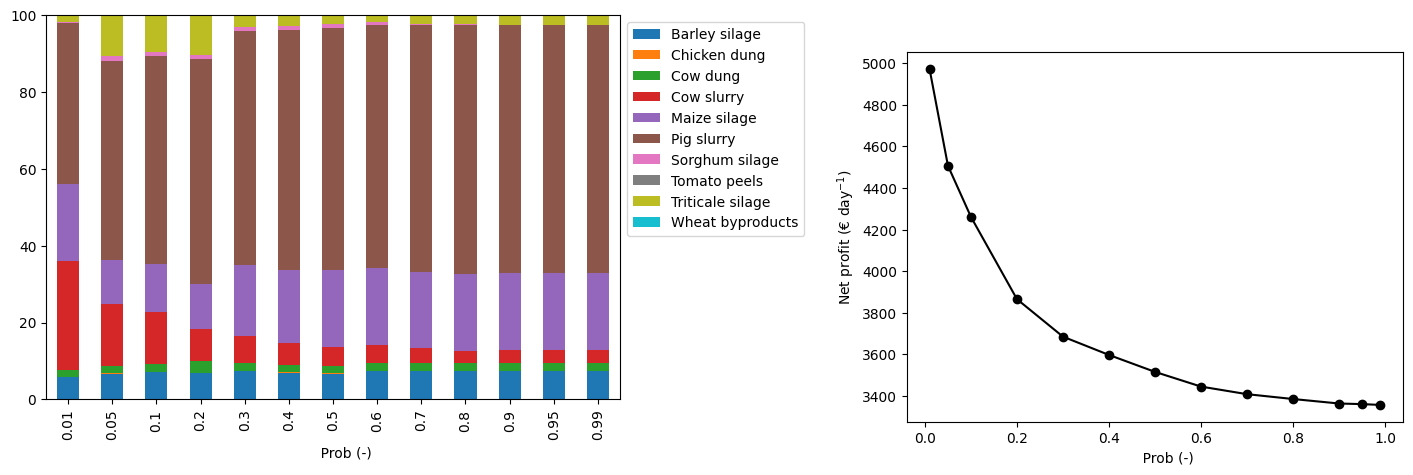
\includegraphics[width=2\columnwidth]{./img/Screening_VarProb_R-LP_20_2024-05-02.png}
 \end{center}
 \caption{Comparison between solutions (left) and objective function values (right) obtained for different value of confidence interval (VaRProb) and HRT=20}
 \label{fig:screenVaR20}
\end{figure*}

\begin{figure*}[htb]
 \begin{center}
  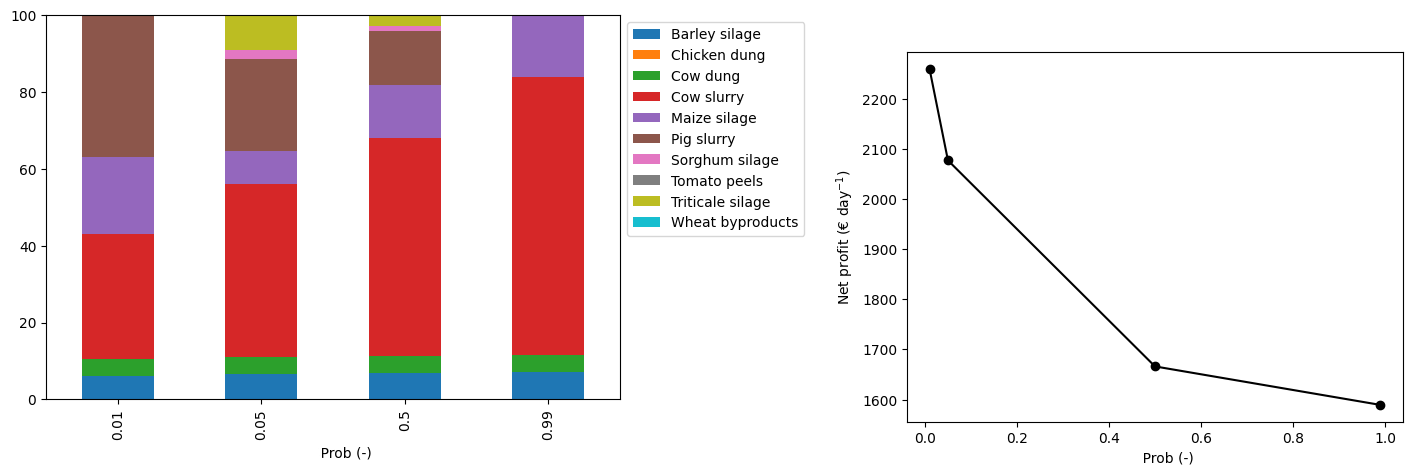
\includegraphics[width=2\columnwidth]{./img/Screening_VarProb_R-LP_50_2024-05-02.png}
 \end{center}
 \caption{Comparison between solutions (left) and objective function values (right) obtained for different value of confidence interval (VaRProb) and HRT=50}
 \label{fig:screenVaR50}
\end{figure*}

%------------------------------------------------------------------------------------

\subsection{Conclusions and further improvements}
\begin{itemize}
    \item For the case under study and with the boundary conditions shaped by the considered data, the exploitation of industrial by-products (es. 'tomato peels' and 'wheat byproducts') in the inflent diet of biomethane plants is not favoured.
    \item Other operational expenditures such as energy self-consumption, etc. can be included to result in more accurate predictions of profit and pushing optimality toward higher values of HRT.
    \item High HRT is suggested for case studies surrounded by high uncertainty. On the other hand, low HRT leads to higher profits. Worst-case realizations for low HRT may result in profits similar to the deterministic problem for high HRT. If non-linear process uncertainties are also considered with the aid of ADM1 simulations of the optimal robust diet, low HRT could be robustly applied to the operation of reactors and higher profits could be achieved.
    \item Price and BMP$_\infty$ uncertainties were proved to have a major impact on the achievable profit. Problem robustification was proved to give conservative results and provide the possibility to derive some interesting considerations on the most profitable and the most robust items/diets.
    \item \textcolor{red}{State someway somehow that we were overly conservative with size parameters and how to improve our estime...jointly BMP and price?}
    \item In this demonstrative problem formulation and solution, N was taken equal to one year for simplicity. Nevertheless, a lower N can be set by decision makers: in that case, the availability and price data must conserve their time dimension when designing uncertainty sets. Indeed, the subset of realizations filtered to the time window of the next selected operating horizon (start time and duration) would need to be considered to adapt the worst case solution to crop and market seasonality. 
    \item Better estimation of BMP(HRT) considering a more realistic behaviour of a continuously fed reactor (different from similarity with batch reactor that was made). 
    A more reliable representation of the operating behaviour of a continously-fed reactor could improve the accuracy of the predictions and favour higher HRTs, in comparison to the assumed similarity with batch-tests for the productivity estime.
    Indeed, instead of Eq.\ref{prodbatch}, Eq. \ref{prodcont} should be used, i.e.
\begin{equation}\label{prodbatch}
    Q_{ch4,i} = BMP_i(HRT) \frac{x_i}{N}
\end{equation}
\begin{equation}\label{prodcont}
    Q_{ch4} = \frac{x_i}{N} \sum_{t=0}^{HRT} E_{CSTR}(t) BMP_i(t) 
\end{equation}
    where \emph{E$_{CSTR}$(t)} is the fraction of effluent material remained in the reactor until time t.
    \item A multi-objective approach can guide further the decision of the operating HRT, trading-off the higher profits of low HRTs with the lower profit variability of high HRTs.   
\end{itemize} 